\documentclass[12pt]{article}

%packages
%\usepackage{latexsym}
\usepackage{graphicx}
\usepackage{color}
\usepackage{amsmath}
\usepackage{dsfont}
\usepackage{placeins}
\usepackage{amssymb}
\usepackage{wasysym}
\usepackage{abstract}
\usepackage{hyperref}
\usepackage{etoolbox}
\usepackage{datetime}
\usepackage{xcolor}
\usepackage{enumerate}
\usepackage{alphalph}
\settimeformat{ampmtime}

%\usepackage{pstricks,pst-node,pst-tree}

%\usepackage{algpseudocode}
%\usepackage{amsthm}
%\usepackage{hyperref}
%\usepackage{mathrsfs}
%\usepackage{amsfonts}
%\usepackage{bbding}
%\usepackage{listings}
%\usepackage{appendix}
\usepackage[margin=1in]{geometry}
%\geometry{papersize={8.5in,11in},total={6.5in,9in}}
%\usepackage{cancel}
%\usepackage{algorithmic, algorithm}

\makeatletter
\def\maxwidth{ %
  \ifdim\Gin@nat@width>\linewidth
    \linewidth
  \else
    \Gin@nat@width
  \fi
}
\makeatother

\definecolor{fgcolor}{rgb}{0.345, 0.345, 0.345}
\newcommand{\hlnum}[1]{\textcolor[rgb]{0.686,0.059,0.569}{#1}}%
\newcommand{\hlstr}[1]{\textcolor[rgb]{0.192,0.494,0.8}{#1}}%
\newcommand{\hlcom}[1]{\textcolor[rgb]{0.678,0.584,0.686}{\textit{#1}}}%
\newcommand{\hlopt}[1]{\textcolor[rgb]{0,0,0}{#1}}%
\newcommand{\hlstd}[1]{\textcolor[rgb]{0.345,0.345,0.345}{#1}}%
\newcommand{\hlkwa}[1]{\textcolor[rgb]{0.161,0.373,0.58}{\textbf{#1}}}%
\newcommand{\hlkwb}[1]{\textcolor[rgb]{0.69,0.353,0.396}{#1}}%
\newcommand{\hlkwc}[1]{\textcolor[rgb]{0.333,0.667,0.333}{#1}}%
\newcommand{\hlkwd}[1]{\textcolor[rgb]{0.737,0.353,0.396}{\textbf{#1}}}%

\usepackage{framed}
\makeatletter
\newenvironment{kframe}{%
 \def\at@end@of@kframe{}%
 \ifinner\ifhmode%
  \def\at@end@of@kframe{\end{minipage}}%
  \begin{minipage}{\columnwidth}%
 \fi\fi%
 \def\FrameCommand##1{\hskip\@totalleftmargin \hskip-\fboxsep
 \colorbox{shadecolor}{##1}\hskip-\fboxsep
     % There is no \\@totalrightmargin, so:
     \hskip-\linewidth \hskip-\@totalleftmargin \hskip\columnwidth}%
 \MakeFramed {\advance\hsize-\width
   \@totalleftmargin\z@ \linewidth\hsize
   \@setminipage}}%
 {\par\unskip\endMakeFramed%
 \at@end@of@kframe}
\makeatother

\definecolor{shadecolor}{rgb}{.77, .77, .77}
\definecolor{messagecolor}{rgb}{0, 0, 0}
\definecolor{warningcolor}{rgb}{1, 0, 1}
\definecolor{errorcolor}{rgb}{1, 0, 0}
\newenvironment{knitrout}{}{} % an empty environment to be redefined in TeX

\usepackage{alltt}
\usepackage[T1]{fontenc}

\newcommand{\qu}[1]{``#1''}
\newcounter{probnum}
\setcounter{probnum}{1}

%create definition to allow local margin changes
\def\changemargin#1#2{\list{}{\rightmargin#2\leftmargin#1}\item[]}
\let\endchangemargin=\endlist 

\newcommand{\errorrv}{\mathcal{E}}
\newcommand{\berrorrv}{\bv{\errorrv}}

%allow equations to span multiple pages
\allowdisplaybreaks

%define colors and color typesetting conveniences
\definecolor{gray}{rgb}{0.5,0.5,0.5}
\definecolor{black}{rgb}{0,0,0}
\definecolor{white}{rgb}{1,1,1}
\definecolor{blue}{rgb}{0.5,0.5,1}
\newcommand{\inblue}[1]{\color{blue}#1 \color{black}}
\definecolor{green}{rgb}{0.133,0.545,0.133}
\newcommand{\ingreen}[1]{\color{green}#1 \color{black}}
\definecolor{yellow}{rgb}{1,1,0}
\newcommand{\inyellow}[1]{\color{yellow}#1 \color{black}}
\definecolor{orange}{rgb}{0.9,0.649,0}
\newcommand{\inorange}[1]{\color{orange}#1 \color{black}}
\definecolor{red}{rgb}{1,0.133,0.133}
\newcommand{\inred}[1]{\color{red}#1 \color{black}}
\definecolor{purple}{rgb}{0.58,0,0.827}
\newcommand{\inpurple}[1]{\color{purple}#1 \color{black}}
\definecolor{backgcode}{rgb}{0.97,0.97,0.8}
\definecolor{Brown}{cmyk}{0,0.81,1,0.60}
\definecolor{OliveGreen}{cmyk}{0.64,0,0.95,0.40}
\definecolor{CadetBlue}{cmyk}{0.62,0.57,0.23,0}

%define new math operators
\DeclareMathOperator*{\argmax}{arg\,max~}
\DeclareMathOperator*{\argmin}{arg\,min~}
\DeclareMathOperator*{\argsup}{arg\,sup~}
\DeclareMathOperator*{\arginf}{arg\,inf~}
\DeclareMathOperator*{\convolution}{\text{\Huge{$\ast$}}}
\newcommand{\infconv}[2]{\convolution^\infty_{#1 = 1} #2}
%true functions

%%%% GENERAL SHORTCUTS

%shortcuts for pure typesetting conveniences
\newcommand{\bv}[1]{\boldsymbol{#1}}

%shortcuts for compound constants
\newcommand{\BetaDistrConst}{\dfrac{\Gamma(\alpha + \beta)}{\Gamma(\alpha)\Gamma(\beta)}}
\newcommand{\NormDistrConst}{\dfrac{1}{\sqrt{2\pi\sigma^2}}}

%shortcuts for conventional symbols
\newcommand{\tsq}{\tau^2}
\newcommand{\tsqh}{\hat{\tau}^2}
\newcommand{\sigsq}{\sigma^2}
\newcommand{\sigsqsq}{\parens{\sigma^2}^2}
\newcommand{\sigsqovern}{\dfrac{\sigsq}{n}}
\newcommand{\tausq}{\tau^2}
\newcommand{\tausqalpha}{\tau^2_\alpha}
\newcommand{\tausqbeta}{\tau^2_\beta}
\newcommand{\tausqsigma}{\tau^2_\sigma}
\newcommand{\betasq}{\beta^2}
\newcommand{\sigsqvec}{\bv{\sigma}^2}
\newcommand{\sigsqhat}{\hat{\sigma}^2}
\newcommand{\sigsqhatmlebayes}{\sigsqhat_{\text{Bayes, MLE}}}
\newcommand{\sigsqhatmle}[1]{\sigsqhat_{#1, \text{MLE}}}
\newcommand{\bSigma}{\bv{\Sigma}}
\newcommand{\bSigmainv}{\bSigma^{-1}}
\newcommand{\thetavec}{\bv{\theta}}
\newcommand{\thetahat}{\hat{\theta}}
\newcommand{\thetahatmle}{\hat{\theta}_{\mathrm{MLE}}}
\newcommand{\thetahatmap}{\hat{\theta}_{\mathrm{MAP}}}
\newcommand{\thetahatmae}{\hat{\theta}_{\mathrm{MAE}}}
\newcommand{\thetahatmmse}{\hat{\theta}_{\mathrm{MMSE}}}
\newcommand{\thetavechatmle}{\hat{\thetavec}_{\mathrm{MLE}}}
\newcommand{\muhat}{\hat{\mu}}
\newcommand{\musq}{\mu^2}
\newcommand{\muvec}{\bv{\mu}}
\newcommand{\muhatmle}{\muhat_{\text{MLE}}}
\newcommand{\lambdahat}{\hat{\lambda}}
\newcommand{\lambdahatmle}{\lambdahat_{\text{MLE}}}
\newcommand{\etavec}{\bv{\eta}}
\newcommand{\alphavec}{\bv{\alpha}}
\newcommand{\minimaxdec}{\delta^*_{\mathrm{mm}}}
\newcommand{\ybar}{\bar{y}}
\newcommand{\xbar}{\bar{x}}
\newcommand{\Xbar}{\bar{X}}
\newcommand{\phat}{\hat{p}}
\newcommand{\Phat}{\hat{P}}
\newcommand{\Zbar}{\bar{Z}}
\newcommand{\iid}{~{\buildrel iid \over \sim}~}
\newcommand{\inddist}{~{\buildrel ind \over \sim}~}
\newcommand{\exchdist}{~{\buildrel exch \over \sim}~}
\newcommand{\approxdist}{~{\buildrel approx \over \sim}~}
\newcommand{\equalsindist}{~{\buildrel d \over =}~}
\newcommand{\loglik}[1]{\ell\parens{#1}}
\newcommand{\thetahatkminone}{\thetahat^{(k-1)}}
\newcommand{\thetahatkplusone}{\thetahat^{(k+1)}}
\newcommand{\thetahatk}{\thetahat^{(k)}}
\newcommand{\half}{\frac{1}{2}}
\newcommand{\third}{\frac{1}{3}}
\newcommand{\twothirds}{\frac{2}{3}}
\newcommand{\fourth}{\frac{1}{4}}
\newcommand{\fifth}{\frac{1}{5}}
\newcommand{\sixth}{\frac{1}{6}}

%shortcuts for vector and matrix notation
\newcommand{\A}{\bv{A}}
\newcommand{\At}{\A^T}
\newcommand{\Ainv}{\inverse{\A}}
\newcommand{\B}{\bv{B}}
\newcommand{\K}{\bv{K}}
\newcommand{\Kt}{\K^T}
\newcommand{\Kinv}{\inverse{K}}
\newcommand{\Kinvt}{(\Kinv)^T}
\newcommand{\M}{\bv{M}}
\newcommand{\Bt}{\B^T}
\newcommand{\Q}{\bv{Q}}
\newcommand{\Qt}{\Q^T}
\newcommand{\R}{\bv{R}}
\newcommand{\Rt}{\R^T}
\newcommand{\Z}{\bv{Z}}
\newcommand{\X}{\bv{X}}
\newcommand{\Xsub}{\X_{\text{(sub)}}}
\newcommand{\Xsubadj}{\X_{\text{(sub,adj)}}}
\newcommand{\I}{\bv{I}}
\newcommand{\Y}{\bv{Y}}
\newcommand{\sigsqI}{\sigsq\I}
\renewcommand{\P}{\bv{P}}
\newcommand{\Psub}{\P_{\text{(sub)}}}
\newcommand{\Pt}{\P^T}
\newcommand{\Pii}{P_{ii}}
\newcommand{\Pij}{P_{ij}}
\newcommand{\IminP}{(\I-\P)}
\newcommand{\Xt}{\bv{X}^T}
\newcommand{\XtX}{\Xt\X}
\newcommand{\XtXinv}{\parens{\Xt\X}^{-1}}
\newcommand{\XtXinvXt}{\XtXinv\Xt}
\newcommand{\XXtXinvXt}{\X\XtXinvXt}
\newcommand{\x}{\bv{x}}
\newcommand{\onevec}{\bv{1}}
\newcommand{\oneton}{1, \ldots, n}
\newcommand{\yoneton}{y_1, \ldots, y_n}
\newcommand{\yonetonorder}{y_{(1)}, \ldots, y_{(n)}}
\newcommand{\Yoneton}{Y_1, \ldots, Y_n}
\newcommand{\iinoneton}{i \in \braces{\oneton}}
\newcommand{\onetom}{1, \ldots, m}
\newcommand{\jinonetom}{j \in \braces{\onetom}}
\newcommand{\xoneton}{x_1, \ldots, x_n}
\newcommand{\Xoneton}{X_1, \ldots, X_n}
\newcommand{\xt}{\x^T}
\newcommand{\y}{\bv{y}}
\newcommand{\yt}{\y^T}
\renewcommand{\c}{\bv{c}}
\newcommand{\ct}{\c^T}
\newcommand{\tstar}{\bv{t}^*}
\renewcommand{\u}{\bv{u}}
\renewcommand{\v}{\bv{v}}
\renewcommand{\a}{\bv{a}}
\newcommand{\s}{\bv{s}}
\newcommand{\yadj}{\y_{\text{(adj)}}}
\newcommand{\xjadj}{\x_{j\text{(adj)}}}
\newcommand{\xjadjM}{\x_{j \perp M}}
\newcommand{\yhat}{\hat{\y}}
\newcommand{\yhatsub}{\yhat_{\text{(sub)}}}
\newcommand{\yhatstar}{\yhat^*}
\newcommand{\yhatstarnew}{\yhatstar_{\text{new}}}
\newcommand{\z}{\bv{z}}
\newcommand{\zt}{\z^T}
\newcommand{\bb}{\bv{b}}
\newcommand{\bbt}{\bb^T}
\newcommand{\bbeta}{\bv{\beta}}
\newcommand{\beps}{\bv{\epsilon}}
\newcommand{\bepst}{\beps^T}
\newcommand{\e}{\bv{e}}
\newcommand{\Mofy}{\M(\y)}
\newcommand{\KofAlpha}{K(\alpha)}
\newcommand{\ellset}{\mathcal{L}}
\newcommand{\oneminalph}{1-\alpha}
\newcommand{\SSE}{\text{SSE}}
\newcommand{\SSEsub}{\text{SSE}_{\text{(sub)}}}
\newcommand{\MSE}{\text{MSE}}
\newcommand{\RMSE}{\text{RMSE}}
\newcommand{\SSR}{\text{SSR}}
\newcommand{\SST}{\text{SST}}
\newcommand{\JSest}{\delta_{\text{JS}}(\x)}
\newcommand{\Bayesest}{\delta_{\text{Bayes}}(\x)}
\newcommand{\EmpBayesest}{\delta_{\text{EmpBayes}}(\x)}
\newcommand{\BLUPest}{\delta_{\text{BLUP}}}
\newcommand{\MLEest}[1]{\hat{#1}_{\text{MLE}}}

%shortcuts for Linear Algebra stuff (i.e. vectors and matrices)
\newcommand{\twovec}[2]{\bracks{\begin{array}{c} #1 \\ #2 \end{array}}}
\newcommand{\threevec}[3]{\bracks{\begin{array}{c} #1 \\ #2 \\ #3 \end{array}}}
\newcommand{\fivevec}[5]{\bracks{\begin{array}{c} #1 \\ #2 \\ #3 \\ #4 \\ #5 \end{array}}}
\newcommand{\twobytwomat}[4]{\bracks{\begin{array}{cc} #1 & #2 \\ #3 & #4 \end{array}}}
\newcommand{\threebytwomat}[6]{\bracks{\begin{array}{cc} #1 & #2 \\ #3 & #4 \\ #5 & #6 \end{array}}}

%shortcuts for conventional compound symbols
\newcommand{\thetainthetas}{\theta \in \Theta}
\newcommand{\reals}{\mathbb{R}}
\newcommand{\complexes}{\mathbb{C}}
\newcommand{\rationals}{\mathbb{Q}}
\newcommand{\integers}{\mathbb{Z}}
\newcommand{\naturals}{\mathbb{N}}
\newcommand{\forallninN}{~~\forall n \in \naturals}
\newcommand{\forallxinN}[1]{~~\forall #1 \in \reals}
\newcommand{\matrixdims}[2]{\in \reals^{\,#1 \times #2}}
\newcommand{\inRn}[1]{\in \reals^{\,#1}}
\newcommand{\mathimplies}{\quad\Rightarrow\quad}
\newcommand{\mathlogicequiv}{\quad\Leftrightarrow\quad}
\newcommand{\eqncomment}[1]{\quad \text{(#1)}}
\newcommand{\limitn}{\lim_{n \rightarrow \infty}}
\newcommand{\limitN}{\lim_{N \rightarrow \infty}}
\newcommand{\limitd}{\lim_{d \rightarrow \infty}}
\newcommand{\limitt}{\lim_{t \rightarrow \infty}}
\newcommand{\limitsupn}{\limsup_{n \rightarrow \infty}~}
\newcommand{\limitinfn}{\liminf_{n \rightarrow \infty}~}
\newcommand{\limitk}{\lim_{k \rightarrow \infty}}
\newcommand{\limsupn}{\limsup_{n \rightarrow \infty}}
\newcommand{\limsupk}{\limsup_{k \rightarrow \infty}}
\newcommand{\floor}[1]{\left\lfloor #1 \right\rfloor}
\newcommand{\ceil}[1]{\left\lceil #1 \right\rceil}

%shortcuts for environments
\newcommand{\beqn}{\vspace{-0.25cm}\begin{eqnarray*}}
\newcommand{\eeqn}{\end{eqnarray*}}
\newcommand{\bneqn}{\vspace{-0.25cm}\begin{eqnarray}}
\newcommand{\eneqn}{\end{eqnarray}}

%shortcuts for mini environments
\newcommand{\parens}[1]{\left(#1\right)}
\newcommand{\squared}[1]{\parens{#1}^2}
\newcommand{\tothepow}[2]{\parens{#1}^{#2}}
\newcommand{\prob}[1]{\mathbb{P}\parens{#1}}
\newcommand{\cprob}[2]{\prob{#1~|~#2}}
\newcommand{\littleo}[1]{o\parens{#1}}
\newcommand{\bigo}[1]{O\parens{#1}}
\newcommand{\Lp}[1]{\mathbb{L}^{#1}}
\renewcommand{\arcsin}[1]{\text{arcsin}\parens{#1}}
\newcommand{\prodonen}[2]{\bracks{\prod_{#1=1}^n #2}}
\newcommand{\mysum}[4]{\sum_{#1=#2}^{#3} #4}
\newcommand{\sumonen}[2]{\sum_{#1=1}^n #2}
\newcommand{\infsum}[2]{\sum_{#1=1}^\infty #2}
\newcommand{\infprod}[2]{\prod_{#1=1}^\infty #2}
\newcommand{\infunion}[2]{\bigcup_{#1=1}^\infty #2}
\newcommand{\infinter}[2]{\bigcap_{#1=1}^\infty #2}
\newcommand{\infintegral}[2]{\int^\infty_{-\infty} #2 ~\text{d}#1}
\newcommand{\supthetas}[1]{\sup_{\thetainthetas}\braces{#1}}
\newcommand{\bracks}[1]{\left[#1\right]}
\newcommand{\braces}[1]{\left\{#1\right\}}
\newcommand{\set}[1]{\left\{#1\right\}}
\newcommand{\abss}[1]{\left|#1\right|}
\newcommand{\norm}[1]{\left|\left|#1\right|\right|}
\newcommand{\normsq}[1]{\norm{#1}^2}
\newcommand{\inverse}[1]{\parens{#1}^{-1}}
\newcommand{\rowof}[2]{\parens{#1}_{#2\cdot}}

%shortcuts for functionals
\newcommand{\realcomp}[1]{\text{Re}\bracks{#1}}
\newcommand{\imagcomp}[1]{\text{Im}\bracks{#1}}
\newcommand{\range}[1]{\text{range}\bracks{#1}}
\newcommand{\colsp}[1]{\text{colsp}\bracks{#1}}
\newcommand{\rowsp}[1]{\text{rowsp}\bracks{#1}}
\newcommand{\tr}[1]{\text{tr}\bracks{#1}}
\newcommand{\rank}[1]{\text{rank}\bracks{#1}}
\newcommand{\proj}[2]{\text{Proj}_{#1}\bracks{#2}}
\newcommand{\projcolspX}[1]{\text{Proj}_{\colsp{\X}}\bracks{#1}}
\newcommand{\median}[1]{\text{median}\bracks{#1}}
\newcommand{\mean}[1]{\text{mean}\bracks{#1}}
\newcommand{\dime}[1]{\text{dim}\bracks{#1}}
\renewcommand{\det}[1]{\text{det}\bracks{#1}}
\newcommand{\expe}[1]{\mathbb{E}\bracks{#1}}
\newcommand{\expeabs}[1]{\expe{\abss{#1}}}
\newcommand{\expesub}[2]{\mathbb{E}_{#1}\bracks{#2}}
\newcommand{\cexpe}[2]{\mathbb{E}\bracks{#1\,|\,#2}}
\newcommand{\indic}[1]{\mathds{1}_{#1}}
\newcommand{\var}[1]{\mathbb{V}\text{ar}\bracks{#1}}
\newcommand{\cov}[2]{\mathbb{C}\text{ov}\bracks{#1, #2}}
\newcommand{\corr}[2]{\mathbb{C}\text{orr}\bracks{#1, #2}}
\newcommand{\se}[1]{\mathbb{S}\text{E}\bracks{#1}}
\newcommand{\seest}[1]{\hat{\mathbb{S}\text{E}}\bracks{#1}}
\newcommand{\bias}[1]{\text{Bias}\bracks{#1}}
\newcommand{\derivop}[2]{\dfrac{\text{d}}{\text{d} #1}\bracks{#2}}
\newcommand{\partialop}[2]{\dfrac{\partial}{\partial #1}\bracks{#2}}
\newcommand{\secpartialop}[2]{\dfrac{\partial^2}{\partial #1^2}\bracks{#2}}
\newcommand{\mixpartialop}[3]{\dfrac{\partial^2}{\partial #1 \partial #2}\bracks{#3}}

%shortcuts for functions
\renewcommand{\exp}[1]{\mathrm{exp}\parens{#1}}
\renewcommand{\cos}[1]{\text{cos}\parens{#1}}
\renewcommand{\sin}[1]{\text{sin}\parens{#1}}
\newcommand{\sign}[1]{\text{sign}\parens{#1}}
\newcommand{\are}[1]{\mathrm{ARE}\parens{#1}}
\newcommand{\natlog}[1]{\ln\parens{#1}}
\newcommand{\oneover}[1]{\frac{1}{#1}}
\newcommand{\overtwo}[1]{\frac{#1}{2}}
\newcommand{\overn}[1]{\frac{#1}{n}}
\newcommand{\oneoversqrt}[1]{\oneover{\sqrt{#1}}}
\newcommand{\sqd}[1]{\parens{#1}^2}
\newcommand{\loss}[1]{\ell\parens{\theta, #1}}
\newcommand{\losstwo}[2]{\ell\parens{#1, #2}}
\newcommand{\cf}{\phi(t)}

%English language specific shortcuts
\newcommand{\ie}{\textit{i.e.} }
\newcommand{\AKA}{\textit{AKA} }
\renewcommand{\iff}{\textit{iff}}
\newcommand{\eg}{\textit{e.g.} }
\newcommand{\st}{\textit{s.t.} }
\newcommand{\wrt}{\textit{w.r.t.} }
\newcommand{\mathst}{~~\text{\st}~~}
\newcommand{\mathand}{~~\text{and}~~}
\newcommand{\ala}{\textit{a la} }
\newcommand{\ppp}{posterior predictive p-value}
\newcommand{\dd}{dataset-to-dataset}

%shortcuts for distribution titles
\newcommand{\logistic}[2]{\mathrm{Logistic}\parens{#1,\,#2}}
\newcommand{\bernoulli}[1]{\mathrm{Bernoulli}\parens{#1}}
\newcommand{\betanot}[2]{\mathrm{Beta}\parens{#1,\,#2}}
\newcommand{\stdbetanot}{\betanot{\alpha}{\beta}}
\newcommand{\multnormnot}[3]{\mathcal{N}_{#1}\parens{#2,\,#3}}
\newcommand{\normnot}[2]{\mathcal{N}\parens{#1,\,#2}}
\newcommand{\classicnormnot}{\normnot{\mu}{\sigsq}}
\newcommand{\stdnormnot}{\normnot{0}{1}}
\newcommand{\uniformdiscrete}[1]{\mathrm{Uniform}\parens{\braces{#1}}}
\newcommand{\uniform}[2]{\mathrm{U}\parens{#1,#2}}
\newcommand{\stduniform}{\uniform{0}{1}}
\newcommand{\geometric}[1]{\mathrm{Geometric}\parens{#1}}
\newcommand{\hypergeometric}[3]{\mathrm{Hypergeometric}\parens{#1,\,#2,\,#3}}
\newcommand{\exponential}[1]{\mathrm{Exp}\parens{#1}}
\newcommand{\gammadist}[2]{\mathrm{Gamma}\parens{#1, #2}}
\newcommand{\poisson}[1]{\mathrm{Poisson}\parens{#1}}
\newcommand{\binomial}[2]{\mathrm{Binomial}\parens{#1,\,#2}}
\newcommand{\negbin}[2]{\mathrm{NegBin}\parens{#1,\,#2}}
\newcommand{\rayleigh}[1]{\mathrm{Rayleigh}\parens{#1}}
\newcommand{\multinomial}[2]{\mathrm{Multinomial}\parens{#1,\,#2}}
\newcommand{\gammanot}[2]{\mathrm{Gamma}\parens{#1,\,#2}}
\newcommand{\cauchynot}[2]{\text{Cauchy}\parens{#1,\,#2}}
\newcommand{\invchisqnot}[1]{\text{Inv}\chisq{#1}}
\newcommand{\invscaledchisqnot}[2]{\text{ScaledInv}\ncchisq{#1}{#2}}
\newcommand{\invgammanot}[2]{\text{InvGamma}\parens{#1,\,#2}}
\newcommand{\chisq}[1]{\chi^2_{#1}}
\newcommand{\ncchisq}[2]{\chi^2_{#1}\parens{#2}}
\newcommand{\ncF}[3]{F_{#1,#2}\parens{#3}}

%shortcuts for PDF's of common distributions
\newcommand{\logisticpdf}[3]{\oneover{#3}\dfrac{\exp{-\dfrac{#1 - #2}{#3}}}{\parens{1+\exp{-\dfrac{#1 - #2}{#3}}}^2}}
\newcommand{\betapdf}[3]{\dfrac{\Gamma(#2 + #3)}{\Gamma(#2)\Gamma(#3)}#1^{#2-1} (1-#1)^{#3-1}}
\newcommand{\normpdf}[3]{\frac{1}{\sqrt{2\pi#3}}\exp{-\frac{1}{2#3}(#1 - #2)^2}}
\newcommand{\normpdfvarone}[2]{\dfrac{1}{\sqrt{2\pi}}e^{-\half(#1 - #2)^2}}
\newcommand{\chisqpdf}[2]{\dfrac{1}{2^{#2/2}\Gamma(#2/2)}\; {#1}^{#2/2-1} e^{-#1/2}}
\newcommand{\invchisqpdf}[2]{\dfrac{2^{-\overtwo{#1}}}{\Gamma(#2/2)}\,{#1}^{-\overtwo{#2}-1}  e^{-\oneover{2 #1}}}
\newcommand{\exponentialpdf}[2]{#2\exp{-#2#1}}
\newcommand{\poissonpdf}[2]{\dfrac{e^{-#1} #1^{#2}}{#2!}}
\newcommand{\binomialpdf}[3]{\binom{#2}{#1}#3^{#1}(1-#3)^{#2-#1}}
\newcommand{\rayleighpdf}[2]{\dfrac{#1}{#2^2}\exp{-\dfrac{#1^2}{2 #2^2}}}
\newcommand{\gammapdf}[3]{\dfrac{#3^#2}{\Gamma\parens{#2}}#1^{#2-1}\exp{-#3 #1}}
\newcommand{\cauchypdf}[3]{\oneover{\pi} \dfrac{#3}{\parens{#1-#2}^2 + #3^2}}
\newcommand{\Gammaf}[1]{\Gamma\parens{#1}}

%shortcuts for miscellaneous typesetting conveniences
\newcommand{\notesref}[1]{\marginpar{\color{gray}\tt #1\color{black}}}

%%%% DOMAIN-SPECIFIC SHORTCUTS

%Real analysis related shortcuts
\newcommand{\zeroonecl}{\bracks{0,1}}
\newcommand{\forallepsgrzero}{\forall \epsilon > 0~~}
\newcommand{\lessthaneps}{< \epsilon}
\newcommand{\fraccomp}[1]{\text{frac}\bracks{#1}}

%Bayesian related shortcuts
\newcommand{\yrep}{y^{\text{rep}}}
\newcommand{\yrepisq}{(\yrep_i)^2}
\newcommand{\yrepvec}{\bv{y}^{\text{rep}}}


%Probability shortcuts
\newcommand{\SigField}{\mathcal{F}}
\newcommand{\ProbMap}{\mathcal{P}}
\newcommand{\probtrinity}{\parens{\Omega, \SigField, \ProbMap}}
\newcommand{\convp}{~{\buildrel p \over \rightarrow}~}
\newcommand{\convLp}[1]{~{\buildrel \Lp{#1} \over \rightarrow}~}
\newcommand{\nconvp}{~{\buildrel p \over \nrightarrow}~}
\newcommand{\convae}{~{\buildrel a.e. \over \longrightarrow}~}
\newcommand{\convau}{~{\buildrel a.u. \over \longrightarrow}~}
\newcommand{\nconvau}{~{\buildrel a.u. \over \nrightarrow}~}
\newcommand{\nconvae}{~{\buildrel a.e. \over \nrightarrow}~}
\newcommand{\convd}{~{\buildrel \mathcal{D} \over \rightarrow}~}
\newcommand{\nconvd}{~{\buildrel \mathcal{D} \over \nrightarrow}~}
\newcommand{\withprob}{~~\text{w.p.}~~}
\newcommand{\io}{~~\text{i.o.}}

\newcommand{\Acl}{\bar{A}}
\newcommand{\ENcl}{\bar{E}_N}
\newcommand{\diam}[1]{\text{diam}\parens{#1}}

\newcommand{\taua}{\tau_a}

\newcommand{\myint}[4]{\int_{#2}^{#3} #4 \,\text{d}#1}
\newcommand{\laplacet}[1]{\mathscr{L}\bracks{#1}}
\newcommand{\laplaceinvt}[1]{\mathscr{L}^{-1}\bracks{#1}}
\renewcommand{\min}[1]{\text{min}\braces{#1}}
\renewcommand{\max}[1]{\text{max}\braces{#1}}

\newcommand{\Vbar}[1]{\bar{V}\parens{#1}}
\newcommand{\expnegrtau}{\exp{-r\tau}}

%%% problem typesetting
\definecolor{darkgrey}{rgb}{0.10,0.10,0.9}

\newcommand{\problem}[1]{\noindent \colorbox{black}{{\color{yellow} \large{\textsf{\textbf{Problem \arabic{probnum}}}}~}} \addtocounter{probnum}{1} \vspace{0.2cm} \\ \iftoggle{professormode}{}{\color{darkgrey}} #1}

\newcommand{\easysubproblem}[1]{\ingreen{\item} \iftoggle{professormode}{}{\color{darkgrey}} [easy] #1 \color{black} }
\newcommand{\intermediatesubproblem}[1]{\inorange{\item} \iftoggle{professormode}{}{\color{darkgrey}} [harder] #1 \color{black} }
\newcommand{\hardsubproblem}[1]{\inred{\item} \iftoggle{professormode}{}{\color{darkgrey}} [difficult] #1 \color{black} }
\newcommand{\extracreditsubproblem}[1]{\inpurple{\item} \iftoggle{professormode}{}{\color{darkgrey}} [E.C.] #1 \color{black} }


\newcommand{\spc}[1]{\iftoggle{professormode}{\\ \vspace{#1cm}}{\\ \vspace{-0.3cm}}}

\makeatletter
\newalphalph{\alphmult}[mult]{\@alph}{26}
\renewcommand{\labelenumi}{(\alphmult{\value{enumi}})}

\newcommand{\support}[1]{\text{Supp}\bracks{#1}}
\newcommand{\mode}[1]{\text{Mode}\bracks{#1}}
\newcommand{\IQR}[1]{\text{IQR}\bracks{#1}}
\newcommand{\quantile}[2]{\text{Quantile}\bracks{#1,\,#2}}

\newcommand{\compexpl}{Compute explicitly as a number rounded to two decimals.}
\newcommand{\exchdist}{~{\buildrel exch \over \sim}~}

\title{Math 390.03-02 / 650.03-01 Spring 2016 \\ Final Examination}
\author{Professor Adam Kapelner}

\date{Wednesday, May 25, 2016}

\begin{document}
\maketitle

\noindent Full Name \line(1,0){410}

\thispagestyle{empty}

\section*{Code of Academic Integrity}

\footnotesize
Since the college is an academic community, its fundamental purpose is the pursuit of knowledge. Essential to the success of this educational mission is a commitment to the principles of academic integrity. Every member of the college community is responsible for upholding the highest standards of honesty at all times. Students, as members of the community, are also responsible for adhering to the principles and spirit of the following Code of Academic Integrity.

Activities that have the effect or intention of interfering with education, pursuit of knowledge, or fair evaluation of a student's performance are prohibited. Examples of such activities include but are not limited to the following definitions:

\paragraph{Cheating} Using or attempting to use unauthorized assistance, material, or study aids in examinations or other academic work or preventing, or attempting to prevent, another from using authorized assistance, material, or study aids. Example: using a cheat sheet in a quiz or exam, altering a graded exam and resubmitting it for a better grade, etc.
\\

\noindent I acknowledge and agree to uphold this Code of Academic Integrity. \\

\begin{center}
\line(1,0){250} ~~~ \line(1,0){100}\\
~~~~~~~~~~~~~~~~~~~~~signature~~~~~~~~~~~~~~~~~~~~~~~~~~~~~~~~~~~~~~~~~~~~~ date
\end{center}

\normalsize

\section*{Instructions}

This exam is 120 minutes and closed-book. You are allowed three pages (front and back) of \qu{cheat sheets.} You may use a graphing calculator of your choice. Please read the questions carefully. If the question reads \qu{compute,} this means the solution will be a number otherwise you can leave the answer in \textit{any} widely accepted mathematical notation which could be resolved to an exact or approximate number with the use of a computer. I advise you to skip problems marked \qu{[Extra Credit]} until you have finished the other questions on the exam, then loop back and plug in all the holes. I also advise you to use pencil. The exam is 100 points total plus extra credit. Partial credit will be granted for incomplete answers on most of the questions. \fbox{Box} in your final answers. Good luck!

\pagebreak

This exam assumes you will be able to compute some answers numerically given a computer. Thus, you can leave your answer in terms of any of the following functions as long as the question does not say \qu{compute explicitly.} However, you must make clear the numerical values that are parameters for these functions.

\begin{table}[htp]
\centering
\small
\begin{tabular}{l | llll}
                 & Quantile  & PMF / PDF  &CDF       & Sampling  \\ 
Distribution &  Function & function         & function &  Function \\ \hline
beta & \texttt{qbeta}($p$, $\alpha$, $\beta$)             
& \texttt{d-}($x$, $\alpha$, $\beta$)
& \texttt{p-}($x$, $\alpha$, $\beta$) 
& \texttt{r-}($\alpha$, $\beta$) \\
betabinomial & \texttt{qbetabinom}($p$, $n$, $\alpha$, $\beta$)              
& \texttt{d-}($x$, $n$, $\alpha$, $\beta$)
& \texttt{p-}($x$, $n$, $\alpha$, $\beta$) 
& \texttt{r-}($n$, $\alpha$, $\beta$) \\

betanegativebinomial & \texttt{qbeta\_nbinom}($p$, $r$, $\alpha$, $\beta$) 
& \texttt{d-}($x$, $r$, $\alpha$, $\beta$)
& \texttt{p-}($x$, $r$, $\alpha$, $\beta$) 
& \texttt{r-}($r$, $\alpha$, $\beta$) \\

binomial & \texttt{qbinom}($p$, $n$, $\theta$) 
& \texttt{d-}($x$, $n$, $\theta$)
& \texttt{p-}($x$, $n$, $\theta$) 
& \texttt{r-}($n$, $\theta$) \\

exponential & \texttt{qexp}($p$, $\theta$) 
& \texttt{d-}($x$, $\theta$) 
& \texttt{p-}($x$, $\theta$) 
& \texttt{r-}($\theta$) \\

gamma & \texttt{qgamma}($p$, $\alpha$, $\beta$) 
& \texttt{d-}($x$, $\alpha$, $\beta$)
& \texttt{p-}($x$, $\alpha$, $\beta$) 
& \texttt{r-}($\alpha$, $\beta$) \\

geometric & \texttt{qgeom}($p$, $\theta$) 
& \texttt{d-}($x$, $\theta$)
& \texttt{p-}($x$, $\theta$) 
& \texttt{r-}($\theta$) \\

inversegamma & \texttt{qinvgamma}($p$, $\alpha$, $\beta$) 
& \texttt{d-}($x$, $\alpha$, $\beta$)
& \texttt{p-}($x$, $\alpha$, $\beta$) 
& \texttt{r-}($\alpha$, $\beta$) \\

negative-binomial & \texttt{qnbinom}($p$, $r$, $\theta$) 
& \texttt{d-}($x$, $r$, $\theta$) 
& \texttt{p-}($x$, $r$, $\theta$) 
& \texttt{r-}($r$, $\theta$) \\

normal (univariate) & \texttt{qnorm}($p$, $\theta$, $\sigma$) 
& \texttt{d-}($x$, $\theta$, $\sigma$)
& \texttt{p-}($x$, $\theta$, $\sigma$) 
& \texttt{r-}($\theta$, $\sigma$) \\

normal (multivariate) & 
& \multicolumn{2}{l}{\texttt{dmvnorm}($\x$, $\muvec$, $\bSigma$)} 
& \texttt{r-}($\muvec$, $\bSigma$) \\

poisson & \texttt{qpois}($p$, $\theta$) 
& \texttt{d-}($x$, $\theta$)
& \texttt{p-}($x$, $\theta$) 
& \texttt{r-}($\theta$) \\

T (standard) & \texttt{qt}($p$, $\nu$) 
& \texttt{d-}($x$, $\nu$) 
& \texttt{p-}($x$, $\nu$)
& \texttt{r-}($\nu$) \\

T (nonstandard) & \texttt{qt.scaled}($p$, $\nu$, $\mu$, $\sigma$) 
& \texttt{d-}($x$, $\nu$, $\mu$, $\sigma$)
& \texttt{p-}($x$, $\nu$, $\mu$, $\sigma$) 
& \texttt{r-}($\nu$, $\mu$, $\sigma$) \\

uniform & \texttt{qunif}($p$, $a$, $b$) 
& \texttt{d-}($x$, $a$, $b$)
& \texttt{p-}($x$, $a$, $b$) 
& \texttt{r-}($a$, $b$) \\


\end{tabular}
\caption{Functions from $\texttt{R}$ (in alphabetical order) that can be used on this exam. The hyphen in colums 3, 4 and 5 is shorthand notation for the full text of the r.v. which can be found in column 2.
}
\label{tab:eqs}
\end{table}

\begin{itemize}
\item The quantile function finds the minimum $x$ which satisfies  $\sum_{x_0 = -\infty}^{x} p(x_0) \geq p$ if the r.v. is discrete or solves for $x$ in the following equation: $\int_{-\infty}^x f(x) dx = p$ if the r.v. is continuous.

\item The PMF / PDF function computes $p(x)$ if the r.v. is discrete or $f(x)$ if the r.v. is continuous.

\item The CDF function calculates the following sum: $\sum_{x_0 = -\infty}^{x} p(x_0)$ if the r.v. is discrete or it calculates the following integral $\int_{-\infty}^x f(x) dx$ if the r.v. is continuous.

\item The sampling function will draw a random realization from the distribution of interest.
\end{itemize}
All other parameters are the function parameters in the density / PMF that you should be familiar with from the class notes (and your cheat sheet)

\pagebreak

\problem This question is about ratings on youtube. Each video which is voted on is either up-voted or down-voted. A video's rating looks like the following:

\begin{figure}[htp]
\centering
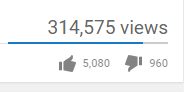
\includegraphics[width=2in]{updown.png}
\end{figure}

\noindent (ignore the number of views). This video for instance has a 5800/(5800 + 960) = 85.8\% approval rating out of 6,760 total votes.  

But there is a question: how should we order videos by approval rating? For example, here is a table of four videos we wish to order about a topic we are interested in:

\begin{table}[htp]
\centering
\begin{tabular}{ccccc}
Video Name & \# Up votes & \# Down votes & $n$ & Approval Rating \\ \hline
A & 5080 & 960 & 6040 & 84.1\% \\
B & 3 & 0 & 3 & 100.0\% \\
C & 25 & 1 & 26 & 96.2\% \\
D & 0 & 1 & 1 & 0.0\%
\end{tabular}
\caption{Table of videos with their youtube ratings.}
\label{tab:ratings}
\end{table}

%xs = c(rbeta(2e4, 3, 1), rbeta(1e4,750, 250))
%%hist(xs, br = 100)
%fw <- fitdist(xs, "beta")
%plot(fw)
%fw



\benum

\subquestionwithpoints{2} Order the movies by name from best to worst using the MLE estimate of its true approval rating.\spc{1} %M1

\subquestionwithpoints{3} Why is what you did in (a) a poor way to order the four movies?\spc{4} %M1

\subquestionwithpoints{1} We are now going to use some previous data to create a prior for the true approval rating. What is this kind of procedure is called? Two words.\spc{3} %M2

Below is a histogram of the approval ratings of $n_0 = 30,000$ videos of which there are more than 200 votes each. The curve displayed atop the histogram is the best fit beta density. I used \texttt{R}'s  \texttt{fitdistrplus} package which creates a fit via the MLE's of $\alpha$ and $\beta$. I include estimates in output from \texttt{R} below the plot. 

\begin{figure}[htp]
\centering
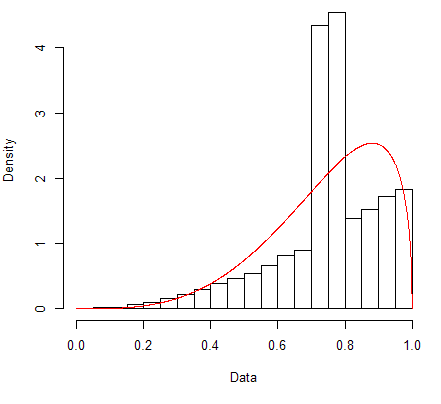
\includegraphics[width=5in]{fitdist.png}
\end{figure}

\begin{verbatim}
Parameters:
       estimate Std. Error
shape1 4.283762 0.03567291
shape2 1.442157 0.01073980
\end{verbatim}

Despite the fact that this fit does not seem to be appropriate, we will use it for now.

\subquestionwithpoints{4} Besides the fact that the curve does not fit the empirical distribution (given by the histogram), what is wrong with the estimates of $\alpha$ and $\beta$ given above? Hint: think about pseudocounts. \spc{5} %M1

\subquestionwithpoints{3} Given that a movie has $n$ total votes and $x$ of those are thumbs up, what is the distribution of the true approval rating $\theta$ given the data coupled with the prior constructed above question (d)?\spc{1} %M1

\subquestionwithpoints{5} Order the movies from best to worst using the Bayesian estimate which minimizes mean squared error. Compute explicitly. No credit unless work is shown.\spc{5} %M1

\subquestionwithpoints{1} We will now attempt to improve the model by improving the prior by modeling the prior as a sum of two beta distributions. What kind of model would this be called? Two words.\spc{1} %M3

\subquestionwithpoints{3} The likelihood function of the two-beta model is below. Remember there are $n_0$ data points in the prior data which I've denoted $y_1, \ldots, y_{n_0}$. Remember that $n$ which denotes the sample size of a single video which we are not estimating yet. 

\beqn
&& \cprob{Y_1, \ldots, Y_{n_0}}{\alpha_1, \beta_1, \alpha_2, \beta_2, \rho} = \prod_{i=1}^{n_0} \rho  f_1(y_i) + (1-\rho) f_2(y_i)\\
&& = \prod_{i=1}^{n_0} \rho  \parens{\oneover{B(\alpha_1, \beta_1)}y_i^{\alpha_1 - 1} (1-y_i)^{\beta_1 - 1}} + (1-\rho) \parens{\oneover{B(\alpha_2, \beta_2)}y_i^{\alpha_2 - 1} (1-y_i)^{\beta_2 - 1}}
\eeqn

Why would estimating $\alpha_1, \beta_1, \alpha_2, \beta_2, \rho$ be difficult if you were to use the MLE method? \spc{8} %M3


\subquestionwithpoints{4} We will instead use the E-M algorithm. Write the likelihood now of the data-augmented model where the $I_i$'s are indicators for the $i$th observation belonging to the $f_1$ distribution. 


\beqn
\cprob{Y_1, \ldots, Y_{n_0}, I_1, \ldots, I_{n_0}}{\alpha_1, \beta_1, \alpha_2, \beta_2, \rho} = \quad\quad\quad\quad\quad\quad\quad\quad\quad\quad\quad\quad\quad\quad\quad\quad\quad\quad\quad\quad\quad\quad\quad\quad\quad\quad\quad\quad\\~\\
 ~~~~~~~~~~~~~~~~~~~~~~~~~~~~~~~~~~~~~~~~~~~~~~~~~~~~~~~~~~~~~~~~~~~~~~~~~~~~~~
\eeqn\spc{2} %M3

\subquestionwithpoints{4} In the E step, write an expression for $\hat{I}_i$ Use hat symbols (the caret on top) to denote estimates. Do not compute. \spc{8} %M3

\subquestionwithpoints{4} In the M step, write an expression for $\hat{\rho}_{MLE}$.  Use hat symbols (the caret on top) to denote estimates. Do not compute.\spc{6} %M3

\subquestionwithpoints{8} Luckily, the \texttt{R} package \texttt{betareg} can run the E-M algorithm for us until it converges. In 33 iterations we got the following: 

\begin{quote}
$\alpha_1 = 2.97$, $\beta_1 = 1.00$, $\alpha_2 = 751.27$, $\beta_2 = 250.44$ and $\rho = 0.666$.
\end{quote} 

Find the Bayesian estimate for video B which minimizes mean squared error for the prior given by these estimates from E-M above. No need to compute explicitly.\spc{9} %M3

\subquestionwithpoints{5} [Extra credit] Video B gets 100 more votes. Without looking at whether they are thumbs up or thumbs down, what is the probability that 65 of them or less are thumbs up? Do not compute explicitly. If you can do this, you may want to work for Google.\spc{12} %M3


%m <- betamix(xs ~ 1 | 1, data = data.frame(xs), k = 2)
%m$flexmix@iter
%mu <- plogis(coef(m)[,1])
%phi <- exp(coef(m)[,2])
%mu
%a <- mu * phi
%b <- (1 - mu) * phi
%a
%b
%m$flexmix@prior
\eenum


\problem This question is about ridge regression. Given $n$ samples from a bivariate distribution, a best fit line was estimated with intercept $b_0$ and slope $b_1$. This estimate is shown as a star on the graph below. The axes represent the entire parameter space $\text{Supp}\bracks{\beta_0} \times \text{Supp}\bracks{\beta_1}$.

\begin{figure}[htp]
\centering
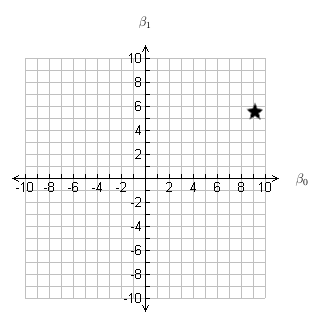
\includegraphics[width=4in]{graph.png}
\end{figure}

\benum

\subquestionwithpoints{3} Imagine a ridge regression was run with ridge penalty $m$ being very large. Mark the graph above with the letter \qu{a} with one place where you think this ridge estimate could be. \spc{0} %M2

\subquestionwithpoints{3} Imagine a ridge regression was run with ridge penalty $m$ being very small. Mark the graph above with the letter \qu{b} with one place where you think this ridge estimate could be. \spc{0} %M2

\subquestionwithpoints{3} Imagine a ridge regression was run with ridge penalty $m = 1$ . Mark the graph above with the letter \qu{c} with one place where you think this ridge estimate could be. \spc{0} %M2

\eenum

\problem We now build a toy Bayesian model where the data points are normal:

\beqn
\Xoneton \exchdist \normnot{\theta}{\sigsq}
\eeqn

\noindent and we have the standard conjugate prior on the mean:

\beqn
\theta~|~\sigsq \sim \normnot{\mu_0}{\frac{\sigsq}{m}}
\eeqn

\noindent but we have the following prior on the variance:

\beqn
\sigsq \sim \gammanot{\overtwo{n_0}}{\beta}
\eeqn

\noindent (note that this is a gamma and not an inverse gamma and the gamma has the same support).

\benum

\subquestionwithpoints{5} Write the posterior exactly below. I have already included the denominator so you do not have to specify that. You only have to specify the numerator. Note: this is an equals sign and not a proportionality sign. You will do the proportionality in the next problem. Hint: I have left it in three pieces for a reason.

\beqn
\cprob{\theta, \sigsq}{\Xoneton} = \oneover{\prob{\Xoneton}} &\times& \parens{\prod_{i=1}^n~~~~~~~~~~~~~~~~~~~~~~~~~~~~~~~~~~~~~~~~~~~~~~~~} \times \\~\\~\\
&& \Bigg(~~~~~~~~~~~~~~~~~~~~~~~~~~~~~~~~~~~~~~~~~~~~~~~~~~~~\Bigg) \times \\~\\~\\
&& \Bigg(~~~~~~~~~~~~~~~~~~~~~~~~~~~~~~~~~~~~~~~~~~~~~~~~~~~~\Bigg)
\eeqn~\spc{0.1}  %M2


\subquestionwithpoints{4} Write the kernel of the posterior below. Use your answer from (a). Collect like terms and simplify.

\beqn
&&\cprob{\theta, \sigsq}{\Xoneton} \propto  ~~~~~~~~~~~~~~~~~~~~~~~~~~~~~~~~~~~~~~~~~~~~~~~~~~~~~~~~~~~~~~~~~~~~~~~~~~~~~~~~~
\eeqn~\spc{4}  %M2

\subquestionwithpoints{2} Is the kernel proportional to a kernel from a known random variable which can be sampled?  (yes / no)  %M2

\subquestionwithpoints{6} Explain in English how you would use grid sampling to sample $n$ draws from the posterior in (a). Say \qu{Step 1,} \qu{Step 2,} etc. Do this problem last! \spc{10.5} %M2

\subquestionwithpoints{3} Despite what you wrote in (d), we are going to attempt to use MCMC to sample from the posterior in (a). Write the kernel of the conditional distribution of $\theta$ given $\sigsq$ and the data below. Use your answer from (b). Then show that it is proportional to a known random variable which can be sampled (make sure to give its parameters).

\beqn
\cprob{\theta}{\Xoneton, ~\sigsq} \propto~~~~~~~~~~~~~~~~~~~~~~~~~~~~~~~~~~~~~~~~~~~~~~~~~~~~~~~~~~~~~~~~~~~~~~~~~~~~~~~~~
\eeqn~\spc{8}  %M3

\subquestionwithpoints{5} Write the kernel of the conditional distribution of $\sigsq$ given $\theta$ and the data below. Use your answer from (b). You can use the notation from class $n\hat{\sigma}^2 := \sum_{i=1}^n (x_i - \theta)^2$ 

\beqn
\cprob{\sigsq}{\Xoneton,~ \theta} \propto~~~~~~~~~~~~~~~~~~~~~~~~~~~~~~~~~~~~~~~~~~~~~~~~~~~~~~~~~~~~~~~~~~~~~~~~~~~~~~~~~
\eeqn~\spc{2} %M3

\subquestionwithpoints{2} Is the kernel proportional to a kernel from a known random variable which can be sampled?  (yes / no) Can you use a Gibbs iteration to sample $\cprob{\sigsq}{\Xoneton,~ \theta}$? (yes / no)%M2

\subquestionwithpoints{2} We will now put together (e) and (f) to create a Metropolis-within-Gibbs sampler. We have $n=50$ samples from the true data generating process. We will use a relatively uninformative prior on $\theta$ which is $\mu_0 = 0$ and $m = 1$. For the gamma prior, we will use an \qu{uninformative} $n_0 = 1$ and $\beta = 1/2$. We will run it for 10,000 iterations. Figure~\ref{fig:conv} shows the first 2,000 iterations. At about what iteration number $t$ did the $\cprob{\theta}{\Xoneton, ~\sigsq}$ chain converge?\spc{0.2}



\subquestionwithpoints{2} At about what  iteration number $t$ did the $\cprob{\sigsq}{\Xoneton, ~\theta}$ chain converge?\spc{0.2} %M3

\subquestionwithpoints{1} Using your answers from (h) and (i), what do you think the burn-in $B$ iteration should be going forward?\spc{0.2} %M3

\subquestionwithpoints{2} Figure~\ref{fig:ac} shows the autocorrelation estimates. At what iteration $t$ would you first be able to thin the $\cprob{\theta}{\Xoneton, ~\sigsq}$ chain?\spc{0.2} %M3





\subquestionwithpoints{2} Figure~\ref{fig:ac} shows the autocorrelation estimates. At what iteration $t$ would you first be able to thin the $\cprob{\sigsq}{\Xoneton, ~\theta}$ chain?\spc{0.2} %M3

\subquestionwithpoints{1} Using your answers from (k) and (l), what do you think the thin-mod value $T$ should be going forward?\spc{0.2} %M3

\subquestionwithpoints{5} Figure~\ref{fig:hist} shows samples from the posterior after the chains were burned and thinned. What integral does the bottom histogram approximate? \spc{1.5} %M3

\subquestionwithpoints{3} Estimate the posterior expectations, $\expe{\theta~|~\Xoneton}$ as well as $\expe{\sigsq~|~\Xoneton}$ using Figure~\ref{fig:hist}. \spc{1.5} %M3


\subquestionwithpoints{2} Use Figure~\ref{fig:hist} to estimate a 95\% credible region for $\theta$. \spc{1} %M3

\subquestionwithpoints{2} Use Figure~\ref{fig:hist} to accept or reject $H_0: \theta \leq 12.5$ by estimating the $p$- value. \spc{1} %M3


\subquestionwithpoints{5} [Extra Credit] What is the probability that 10 new observations will have an average greater than 14? Write an algorithm below that would approximate this. You can reference figure~\ref{fig:hist} in your answer. \spc{16}

\eenum


\begin{figure}[htp]
\centering
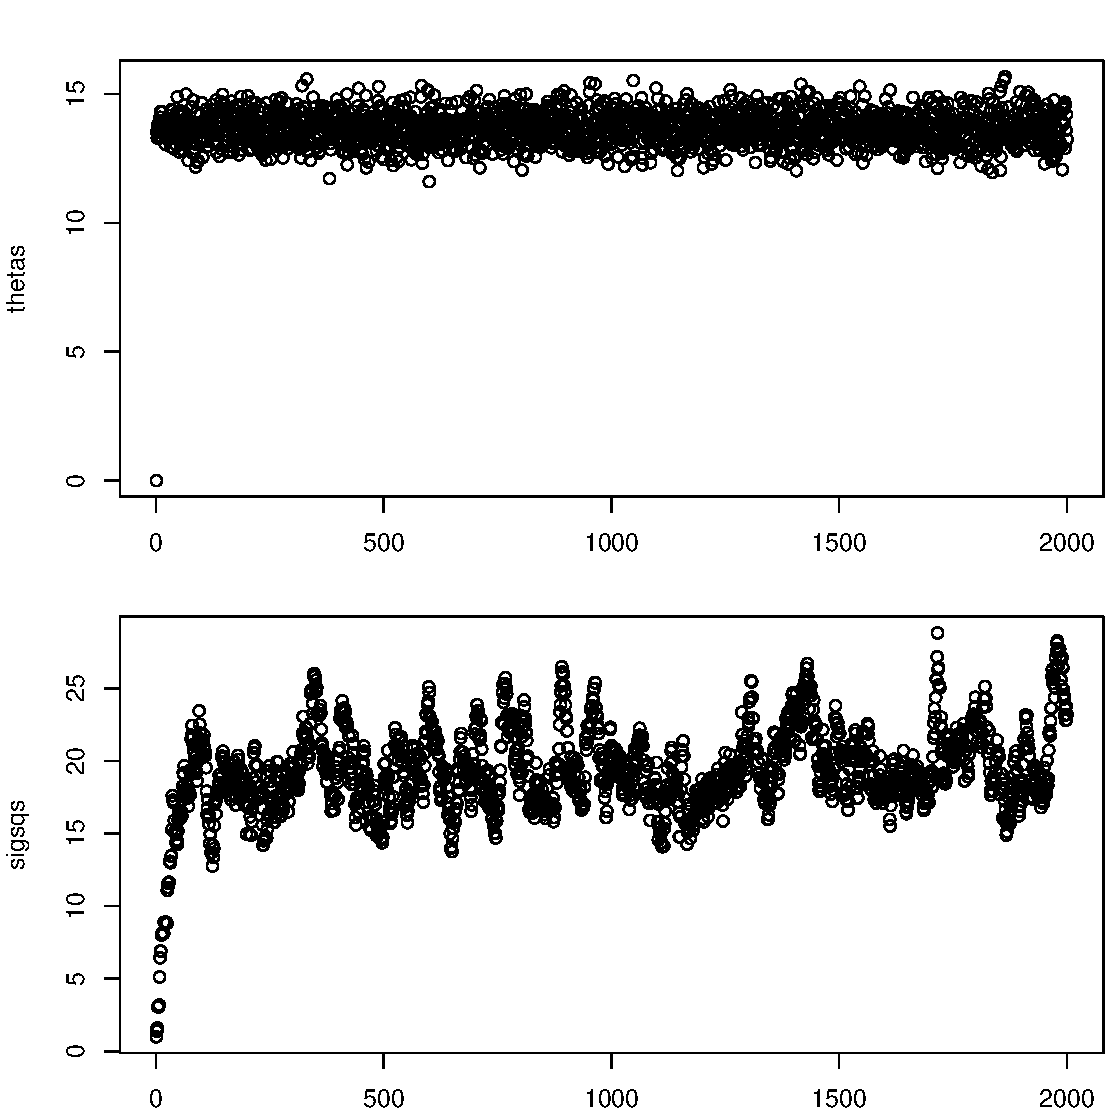
\includegraphics[width=7in]{conv}
\caption{First 2,000 iterations of the Metropolis-within-Gibbs sampler for this data.}
\label{fig:conv}
\end{figure} %M3

\begin{figure}[htp]
\centering
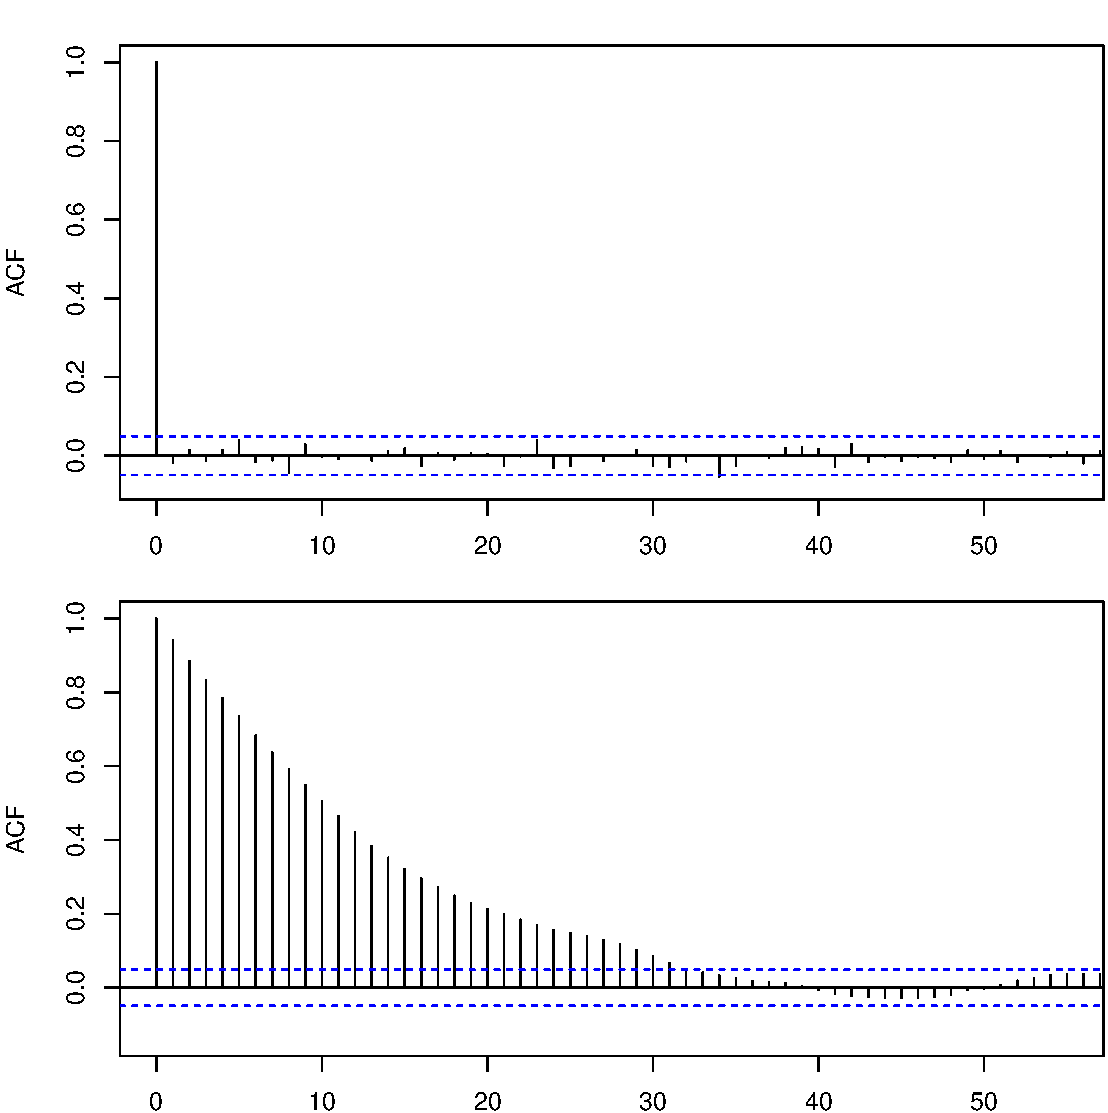
\includegraphics[width=7in]{ac}
\caption{Autocorrelation plots of the Metropolis-within-Gibbs sampler for this data.}
\label{fig:ac}
\end{figure}

\begin{figure}[htp]
\centering
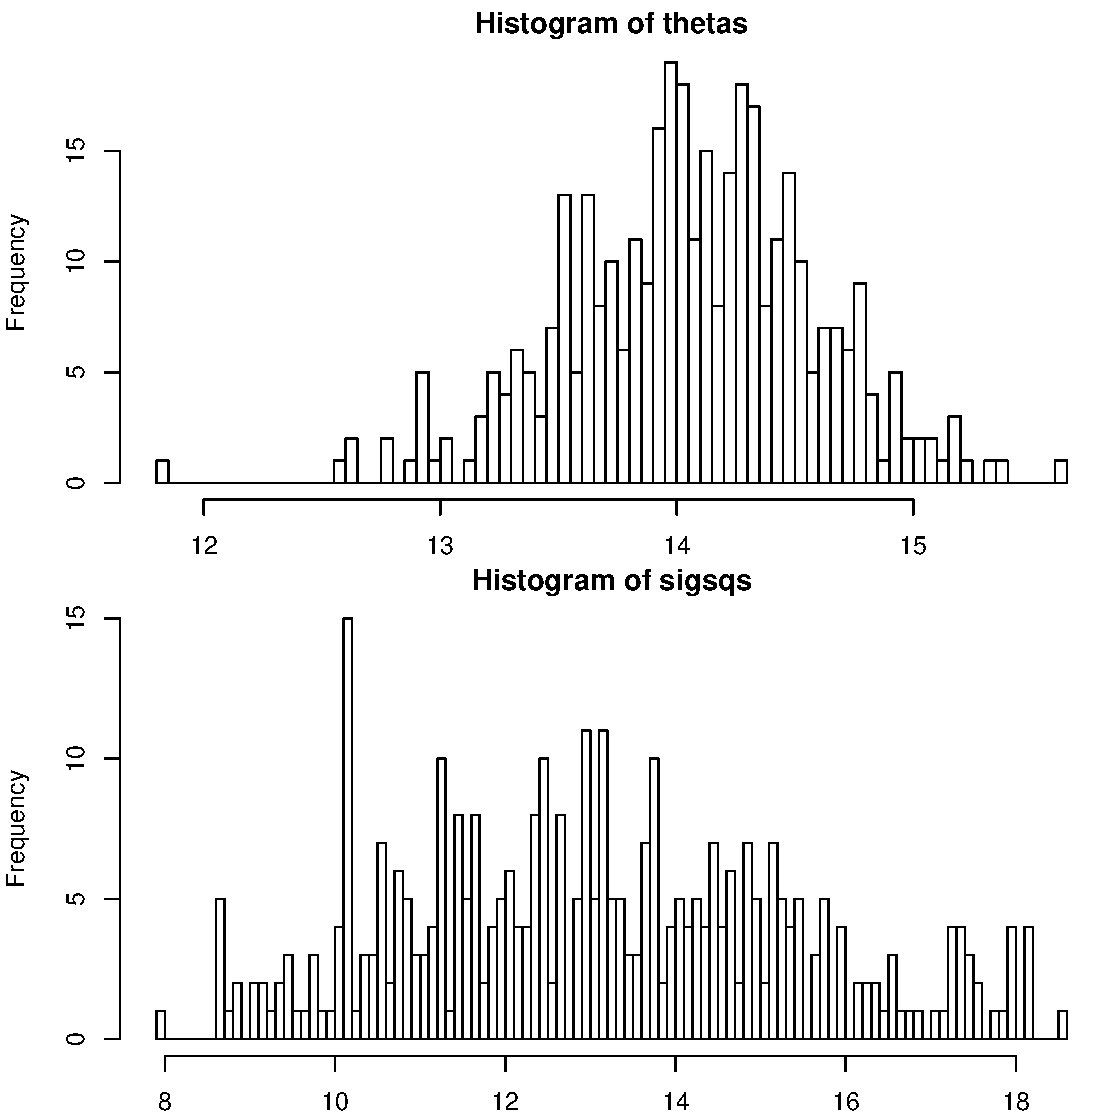
\includegraphics[width=7in]{hist}
\caption{Histograms of the Metropolis-within-Gibbs sampler for this data.}
\label{fig:hist}
\end{figure}


\end{document}






\problem This question is about midair collisions over American soil --- an event which whose probabilities were first predicted using Bayesian methods as we learned about in McGrayne's book.

\begin{figure}[htp]
\centering
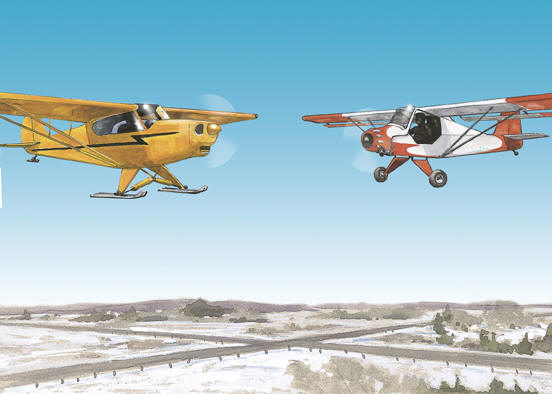
\includegraphics[width=2in]{midair.jpg}
\end{figure}

Since there are on the order of 10's of millions of flight hours per year and collisions are rare, this can be modeled using the Poisson random variable. Table~\ref{tab:collision} shows collision data in United States airspace by year from 1969 - 1978.

\begin{table}[htp]
\centering
\begin{tabular}{cc}
Year & Number of Collisions \\ \hline
1969 &23 \\
1970 &32 \\
1971 &27 \\
1972 &24 \\
1973 &24 \\
1974 &32 \\
1975 &28 \\
1976 &30 \\
1977 &34 \\
1978 &33 \\
\end{tabular}
\caption{Official US Midair collision data for $n=10$ years from 1969-1978}
\label{tab:collision}
\end{table}




\benum

\subquestionwithpoints{3} The model we're using is $X_1, \ldots, X_n \exchdist \poisson{\theta}$ where each $X_i$ is the model for number of collisions in a given year. Is this a realistic model? Why or why not? There is no \qu{correct} answer here but I expect you to defend whatever answer you write using the concepts we discussed in class.\spc{4}

\subquestionwithpoints{4} Despite what you wrote in (a), assume the model is exchangeable for the rest of the problem. We are interested in inference for $\theta$ and we have no subjective prior opinion so we need to employ an objective prior for $\theta$. However, $\theta$ will determine insurance rates and people's decision to fly, so we're really interested in some cost function $c(\theta)$ which will be monotonic but complicated. Which objective prior should we use to avoid getting different answers when new $c$ functions are considered? Make sure you write $\theta \sim$ something below and make sure you specify the parameters as numbers.\spc{2}

\subquestionwithpoints{5} Given the data in Table~\ref{tab:collision} and the prior in (b), provide a 99\% credible region for the true mean number of midair collisions from 1969-1978. Use the notation from Table~\ref{tab:eqs} but do not solve numerically.\spc{4}

\subquestionwithpoints{5} Given the data in Table~\ref{tab:collision} and the prior in (b), calculate the probability that in 1979 we would see 36 or more midair collisions. Use the notation from Table~\ref{tab:eqs} but do not solve numerically.\spc{7}

\subquestionwithpoints{3} We would like to check if our model is valid using a graphical check. So we look at our dataset (which we denote $x$) against samples from $\cprob{X^*}{X = x}$ where the dimension of $X^*$ is the same as the dataset, $n$. Here are a few below. The real data is colored black and the posterior samples are in grey.

\begin{figure}[htp]
\centering
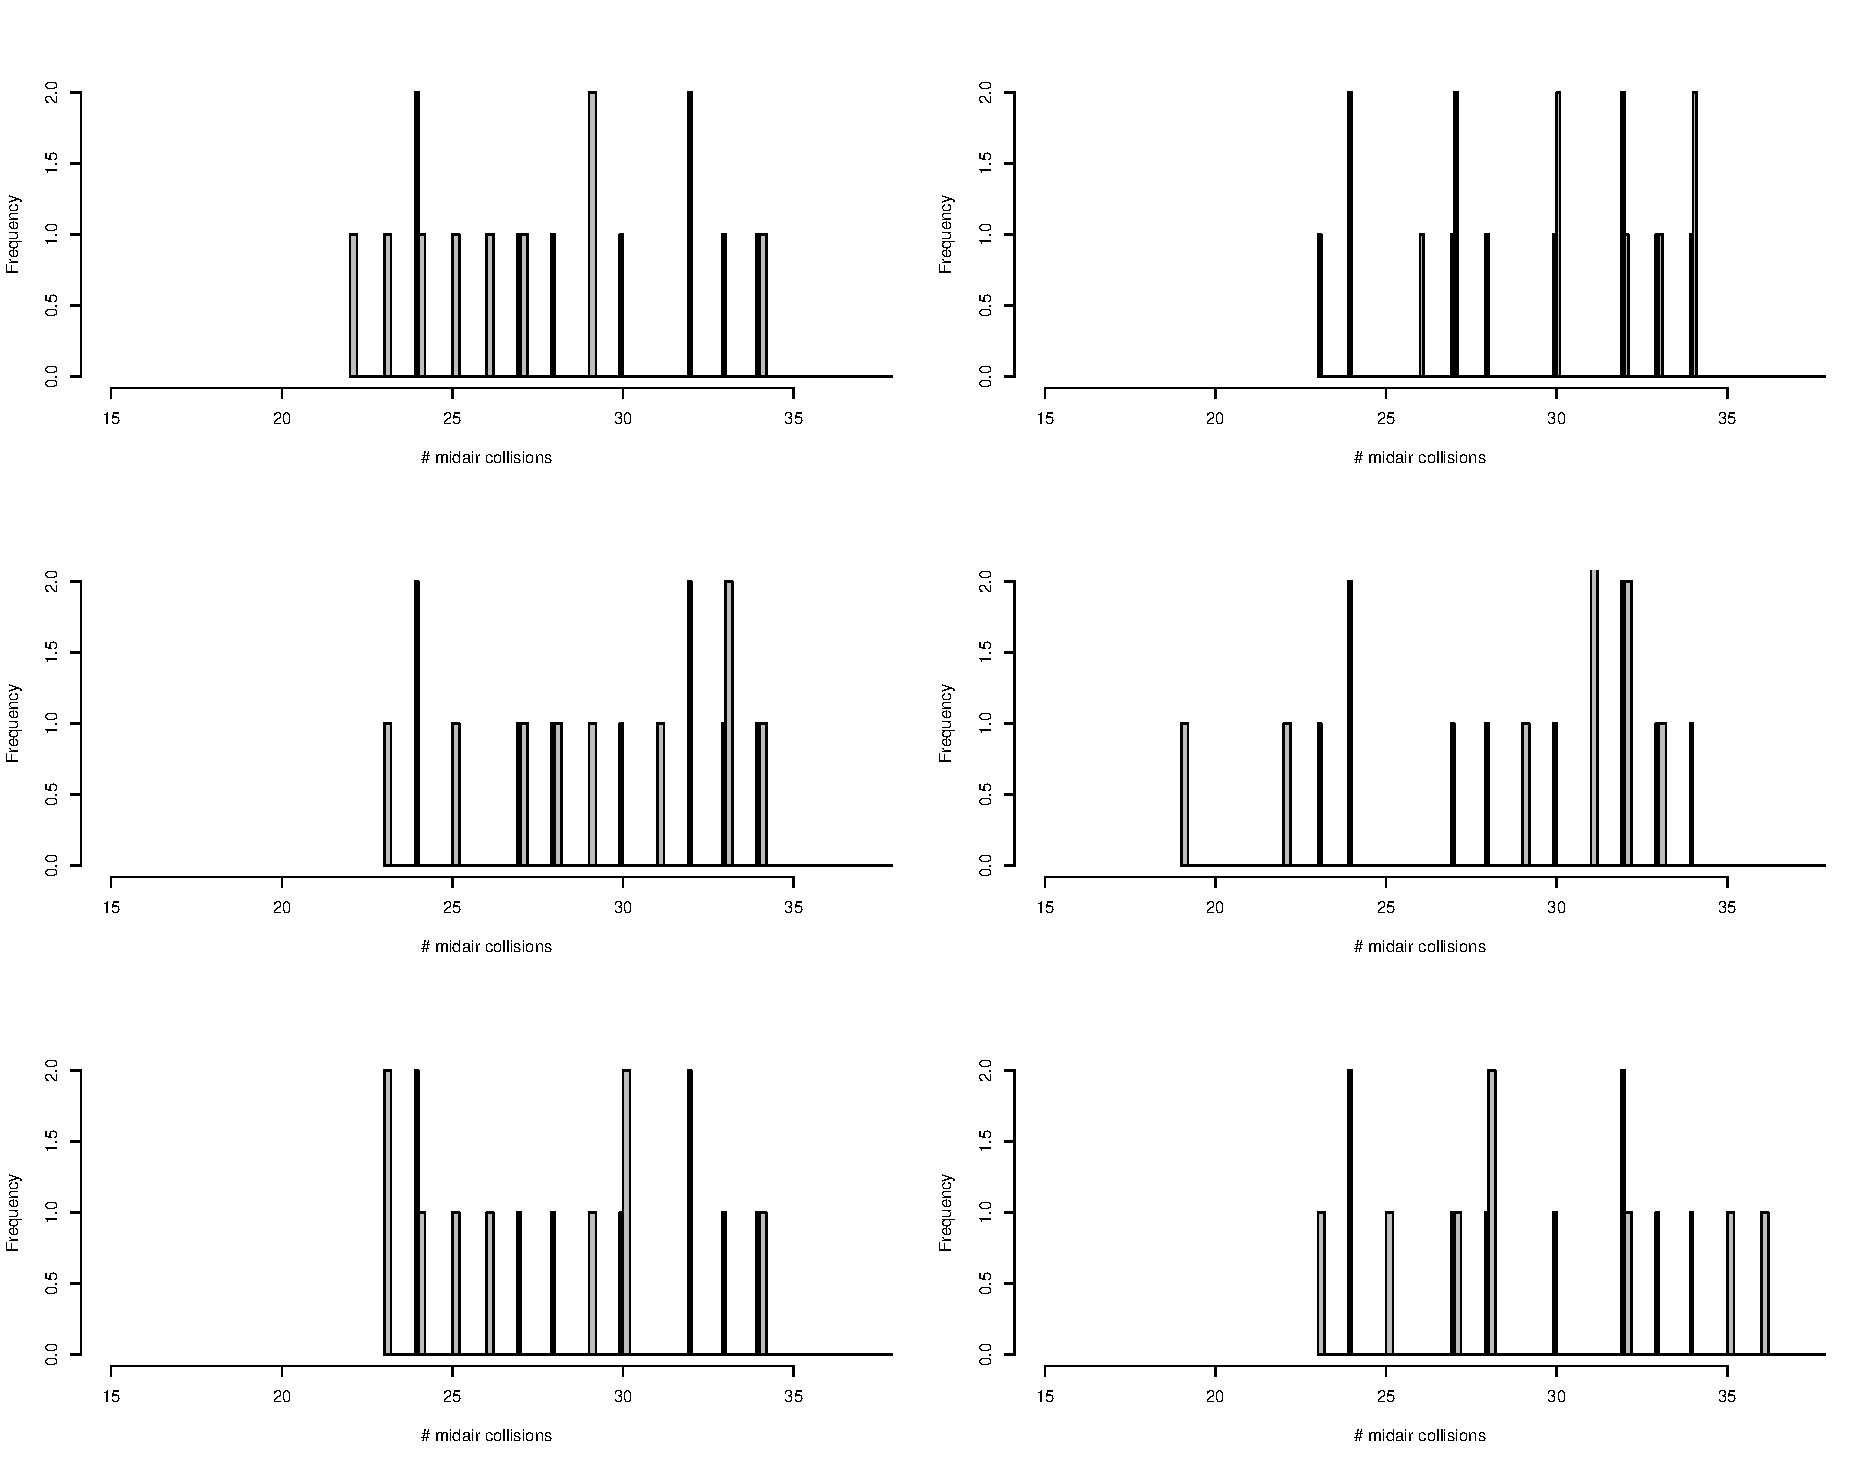
\includegraphics[width=7in]{ppp}
\end{figure}

Does this model seem to be appropriate for the data? Why or why not?\spc{7}

\subquestionwithpoints{3} [Extra Credit] Exactly how did I generate those figures? For any one of the above six figures, write the steps necessary. (All the figures are identical modulo random sampling). Use the notation from Table~\ref{tab:eqs}.\spc{6}

%cs = c(23,32,27,24,24,32,28,30,34,33)
%sumxis = sum(cs)
%n = length(cs)
%alpha = 0.5
%beta = 0
%par(mfrow = c(3, 2))
%for (i in 1 : 6){
%	theta = rgamma(1, sumxis + alpha, n + beta)
%	xstars = rpois(n, theta)
%	hist(cs, br = 100, col = "black", xlim = c(15, 37), xlab = "# midair collisions", main = "")
%	hist(xstars + .0001, br = 100, col = "grey", add = TRUE)
%}

\eenum


\problem We want to predict sale price of new cars based on fuel efficiency measured in miles per gallon (MPG). 

\begin{figure}[htp]
\centering
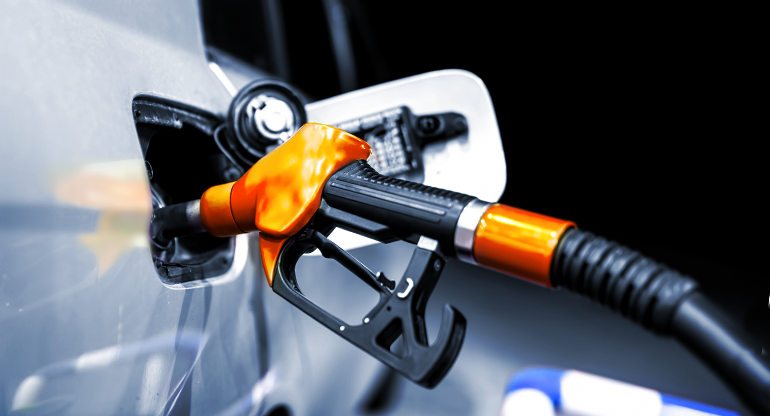
\includegraphics[width=2.5in]{fuel.png}
\end{figure}

Table~\ref{tab:mpgs} displays sample data for a sample of 10 Japanese cars.

\begin{table}[htp]
\centering
\begin{tabular}{c|c}
Fuel efficiency & Price New \\
(nearest MPG) & (nearest \$1000) \\ \hline
31 &23 \\
31 &29 \\
30 &27 \\
29 &25 \\
30 &28 \\
30 &27 \\
28 &28 \\
32 &29 \\
29 &26 \\
28 &27 \\
\end{tabular}
\caption{Fuel Efficiency and sale price for 10 Japanese cars}
\label{tab:mpgs}
\end{table}


%n=10
%xs = rnorm(n, 30, 1)
%ys = 5 + 0.8 * xs + rnorm(n, 0, .2)
%summary(lm(ys~xs))
%r = cor(xs, ys)
%sdx = sd(xs)
%sdy = sd(ys)
%xbar = mean(xs)
%ybar = mean(ys)


\benum
\subquestionwithpoints{3} If you were building a prediction model for this problem using data such as the data pictured in Table~\ref{tab:mpgs}, what would the $x$ variable be and what would the $y$ variable be? \spc{2}

\subquestionwithpoints{3} On a similar dataset of size $n = 10$, you calculate $\xbar = 30.08$, $\ybar = 29.01$, $r = 0.946$, $s_x = 0.609$ and $s_y = 0.534$. Use this information to determine the least squares estimates for the best fit line. Recall, $b_1 = r\frac{s_y}{s_x}$. \spc{2}

\subquestionwithpoints{3} Is your answer in (b) dependent on assuming the OLS assumptions? Yes / no. Circle the answer.  \spc{0} \vspace{-0.7cm}

\subquestionwithpoints{3} If you were to use a ridge penalty to determine your best fit line, would your intercept be smaller or larger? Circle the answer.  \spc{0} \vspace{-0.7cm}

\subquestionwithpoints{3} If you were to use a ridge penalty to determine your best fit line, would your slope be smaller or larger? Circle the answer.  \spc{0} \vspace{-0.7cm}

\subquestionwithpoints{3} Would you be able to use logistic regression to predict car price? \\ Yes / no. Circle the answer.  \spc{0} \vspace{-0.7cm}

\subquestionwithpoints{6} Let's say you have no prior information on where your intercept should be, but prior information on where your slope should be indexed by $m$ such that $\beta_1 \sim \normnot{0}{\sigsq / m}$. Find the most parsimonious kernel for the posterior of $\cprob{\beta_1, \beta_0}{\X, y, \sigsq}$ assuming the OLS assumptions. Show your steps for partial credit. \spc{9}

\subquestionwithpoints{3} [Extra credit] Solve for this \qu{half ridge} estimator (denote it $B_{\tilde{R}}$) proposed in (f). Hint: the ridge estimator is $B_R := \inverse{\XtX +m I_p} \Xt Y$.\spc{6}

\subquestionwithpoints{3} [Extra credit] If you were using a Bayesian model for $\beta$ with the OLS assumptions and the ridge prior, how would you estimate $\expe{\norm{\beta}^2~|~\X, y, \sigsq}$? Hint: use the Monte Carlo / sampling concept we learned about in class and function(s) in Table~\ref{tab:eqs}.\spc{6}

\subquestionwithpoints{3} [Extra credit] Why does ridge regression frequently perform better than regular least squares regression on new observations?\spc{6}

\eenum

\problem This question is about building models for the prices of cars.

\begin{figure}[htp]
\centering
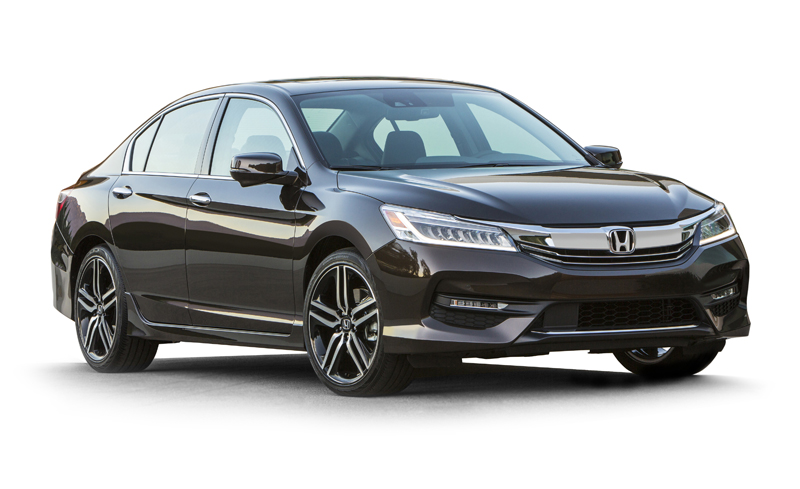
\includegraphics[width=2.7in]{accord.jpg}
\end{figure}

The 2016 Honda Accord sells at many different dealerships in New York City but sell it for more and some for less. We'll assume that the final negotiated price is distributed normally because it's most likely the sum of many different negotiation factors.

Our goal here is to determine the mean price at a certain car dealership in Astoria that people have been saying is \qu{too cheap} and if it's too cheap, Honda corporate may wish to investigate.

Below are the sample average selling prices (in USD) of Honda Accords from 16 other car dealerships also in the NYC area that serve as a comparison:

\begin{verbatim}
22889.80 21159.16 23796.71 19132.65 23450.63 24088.28 19852.37 21306.45
24434.05 23150.34 21690.09 20640.79 21973.45 21984.48 22326.00 22239.98
\end{verbatim}

\benum

\subquestionwithpoints{4} The average of the above prices is 22132.20 and the standard deviation is 1496.30. Create a prior distribution using empirical Bayes for the mean price at the Astoria car dealership. Assume we are using the normal-normal model. \spc{3}

\subquestionwithpoints{4} Assume that each Accord's price at the Astoria dealership is normal and exchangeable. Is this a good model? Why or why not? There is no \qu{correct} answer here but I expect you to defend whatever answer you write using the concepts we discussed in class. \spc{5}

\subquestionwithpoints{4} Despite what you wrote in (b), assume the model is exchangable for the rest of the problem. The nationwide average standard deviation for a Honda Accord selling price we're going to assume is $\sigma = \$1000$, an assumption we will relax later. Given a sample with average $\xbar$ and sample size $n$, what is the distribution of the mean price of a car from this shady Astoria dealership? Assume your prior from (a).\spc{5}

\subquestionwithpoints{4} You and your colleague go down to the Astoria dealership undercover and ask to buy a Honda. After much negotiation, they will sell it to you for \$19,000 and they will sell it to your colleague for \$18,200 but they sense something suspicious so you hesitate to send another one of your guys down there to do another faux negotiation. Unfortunately, we're going to have to estimate the mean with just $x_1=19000$ and $x_2 = 18200$. What is your best guess of the mean price of Honda Accords sold here? Assume your prior from (a). \compexpl \spc{2}

\subquestionwithpoints{4} What is the shrinkage value (which we have been denoting $\rho$) for this estimate? \compexpl\spc{8}

\subquestionwithpoints{6} Based on this data, we wish to test if this dealership is selling Honda Accords below the manufacturer sugested retail price (MSRP) of \$22,205 --- if so, they would be subject to a fine. Calculate a $p$-value for this test below by using notation from Table~\ref{tab:eqs} but do not solve numerically.\spc{6}

\subquestionwithpoints{6} What is the probability I get a really good deal --- that I can buy a car from these Astoria people for under \$17,000? Use the notation from Table~\ref{tab:eqs} but do not solve numerically.\spc{3}


\subquestionwithpoints{4} If you were to estimate (g) without knowledge that $\sigma = \$1000$ but instead use \textit{an} uninformative prior (not necessarily \qu{the} uniformative prior) for $\sigsq$, would the probability of getting the same really good deal be greater than, less than or equal to your answer in (g)? Explain why. \spc{8}


\subquestionwithpoints{6} We will continue to not rely on the nationwide average of $\sigma = \$1000$. Here, instead of an uninformative prior, use the data from the problem header to \textit{estimate} a conjugate prior for $\sigsq$. Pretend those 16 car dealerships are cars themselves. Be clear about everything your estimate relies on. Round the parameters to two decimal points.\spc{4}

\subquestionwithpoints{4} We want to use the answer from (i) to fit a \textit{conjugate} normal-normal model (with $\sigsq$ unknown). This requires solving for $m$ in the $\cprob{\theta}{\sigsq}$ prior. So we set $s^2$ from (a) equal to $\sigsq / m$ and solve for $m$ and we get $m$ = 0.45 rounded to the nearest two digits. What is our prior on $\theta, \sigsq$ now? You can notate your answer in terms of standard densities and you do not have to simplify it to a kernel. \spc{4}

\subquestionwithpoints{6} Given the data in (d) which is $x_1=19000$ and $x_2 = 18200$, what is your best guess of the mean price of Honda Accords sold here? Assume your conjugate prior from (j). Round to the nearest cent. \spc{2}


\subquestionwithpoints{4} If you were to answer (k) but this time assume an independent prior for $\theta$ from (a) and independent prior for $\sigsq$ from (i) and \textit{not} use the conjugate prior in (k), you would not be able to simply compute an estimate of mean price. Explain one way in which you could go about estimating this mean now. Provide one sentence of explanation \textit{only}. I am not looking for you to do any computation or describe a computer program. \spc{6}


\eenum





\end{document}


\begin{figure}[htp]
\centering
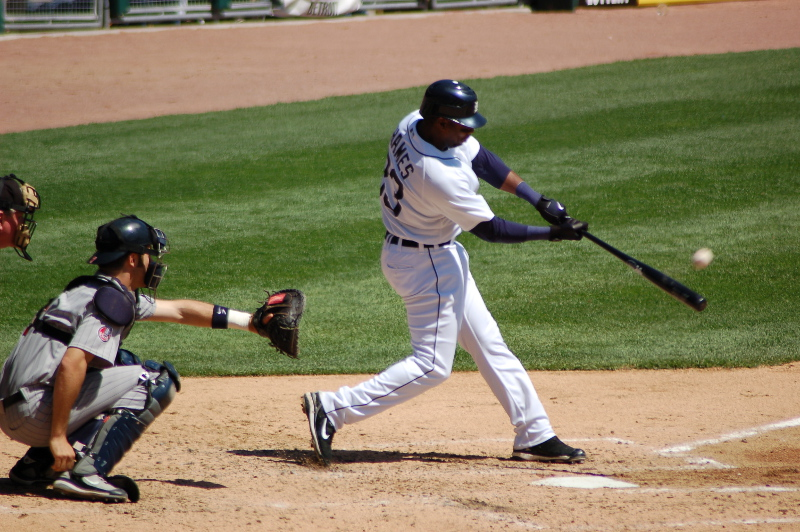
\includegraphics[width=4in]{baseball.jpg}
\end{figure}

\end{document}

\problem This question is about \qu{batting averages} in baseball.

\begin{figure}[htp]
\centering
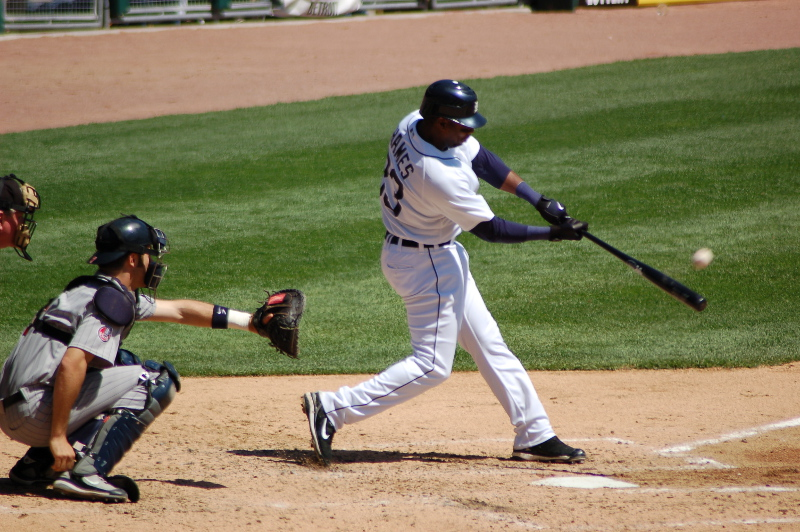
\includegraphics[width=4in]{baseball.jpg}
\end{figure}

\noindent Every hitter's \emph{sample} batting average (BA) is defined as:

\beqn
BA := \frac{\text{sample \# of hits}}{\text{sample \# of at bats}}
\eeqn

In this problem we care about estimating a hitter's \emph{true} batting average which we call $\theta$. Each player has a different $\theta$ but we focus in this problem on one specific player. In order to estimate the player's true batting average, we use the sample batting average as defined above. 

\benum
\subquestionwithpoints{2} For the remainder of the problem, we assume that each at bat (for any player) are \emph{conditionally} $\iid$ based on the players' true batting average, $\theta$. So if a player has $n$ at bats, then each successful hit in each at bat can be modeled via

\beqn
X_1~|~\theta, ~X_2~|~\theta, \ldots, ~X_n~|~\theta \iid \bernoulli{\theta}.
\eeqn

Under this model above, if the player had $n=4$ at bats, would the $\prob{X_3,X_2,X_4,X_1}$ be equal to the $\prob{X_1,X_2,X_3,X_4}$? Yes / no. \spc{1}

\subquestionwithpoints{3} If the player had $n=4$ at bats and $\sum_{i=0}^n x_i=0$ hits, compute $\thetahatmle$.\spc{2}

\subquestionwithpoints{4} Compute a frequentist confidence interval for $\theta$ given the data in (b).\spc{2}


\subquestionwithpoints{3} Describe in English the main problem with the interval in (c).\spc{2}

\subquestionwithpoints{2} Set the following prior: $\theta \sim \stduniform$. Is this an informative prior for the true batting average? Yes/no \spc{1}

\subquestionwithpoints{5} Given the prior in (e) and the data in (b), find the posterior distribution of this player's true batting average.\spc{3}

\subquestionwithpoints{3} Based on your posterior distribution in (f), give your best estimate to the value of $\theta$ which minimizes squared error loss.\spc{3}

\subquestionwithpoints{2} Based on your posterior distribution in (f), describe using an integral or \texttt{R}-language expression your best estimate to the value of $\theta$ which minimizes absolute error loss but do not compute.\spc{4}

\subquestionwithpoints{4} Based on your posterior distribution in (f), give your best estimate to the value of $\theta$ using the posterior mode.\spc{2}

\subquestionwithpoints{5} Find an integral expression for the probability this hitter bats above a 300 batting average (which means the true batting average is 0.3 or greater). Do not compute. \spc{2}

\subquestionwithpoints{5} Assuming you have access to \texttt{R} and its function \texttt{qbeta}, give the 95\% credible region for $\theta$. The three arguments for \texttt{qbeta} are (1) quantile (2) alpha and (3) beta. Then, provide an interpretation for this interval. \spc{2}

\subquestionwithpoints{3} What would the Jeffrey's prior be in our model situation described in (a)? \spc{1}

\subquestionwithpoints{2} Would the posterior under the Haldane prior be proper given the data in (b)? Yes / No. \spc{0.5}

\subquestionwithpoints{5} The batting average is \textit{only} measured as the batting average and never logged or transformed. Would there be any value in using the Jeffrey's prior instead of the prior in (e)? Discuss. \spc{5}


\subquestionwithpoints{5} Looking at the entire dataset for 6,061 batters who had 100 or more at bats, I fit a beta function to the sample batting averages and estimated $\alpha = 42.3$ and $\beta = 127.7$ (which we called \qu{empirical Bayes} estimates in class). Consider building a prior from this estimate as

\beqn
\theta \sim \betanot{42.3}{127.7}.
\eeqn

Would a prior based on these hyperparameter estimates be \qu{objective}? Yes / No. Why? \spc{3}

\subquestionwithpoints{2} Is the prior from (o) considered a \qu{conjugate prior}? Yes / No.\spc{0.5}

\subquestionwithpoints{3} Using the prior from (o), find the $\thetahatmmse$ without considering the data whatsoever. Round to 3 digits. \spc{3}

\subquestionwithpoints{4} Using the prior from (o) and the data from (b), find the posterior $\thetahatmmse$. Round to 3 digits. \spc{2}

\subquestionwithpoints{5} The posterior estimate from (q) is different from the frequentist estimate in (b) due to shrinkage. What is the proportion of shrinkage for the posterior estimate in (q)? We denoted this as $\rho$ in class. Round to 3 digits. \spc{3}

\subquestionwithpoints{4} [Extra Credit] Using the Bayesian CLT, compute a 95\% credible region for $\theta$ for the data in (b) and the prior in (o). Round to 3 digits. \spc{3}

\subquestionwithpoints{3} Based on the data in (b) and the prior in (o), what is the probability this batter gets a hit on his next at bat? \spc{3}

\subquestionwithpoints{5} Based on the data in (b) and the prior in (o), write an exact expression for the batter getting 14 or more hits on the next 20 at bats. You can leave your answer in terms of the beta function. Do not compute explicitly. \spc{5}

\subquestionwithpoints{6} Based on the data in (b) and the prior in (o), find the kernel of the distribution for the number of hits this batter gets in the next $m$ at bats. Partial credit is given. \spc{3}

\subquestionwithpoints{2} Based on the data in (b) and the prior in (o), the joint posterior predictive distribution for $n=4$ looks like as follows. 

%library(VGAM)
%barplot(dbetabinom.ab(0 : 4, 4, shape1 = 42.3 + 0, shape2 = 127.7 + 4), names = 0 : 4, xlab = "X* (# hits)", ylab = "prob(X*|X)")
\begin{figure}[htp]
\centering
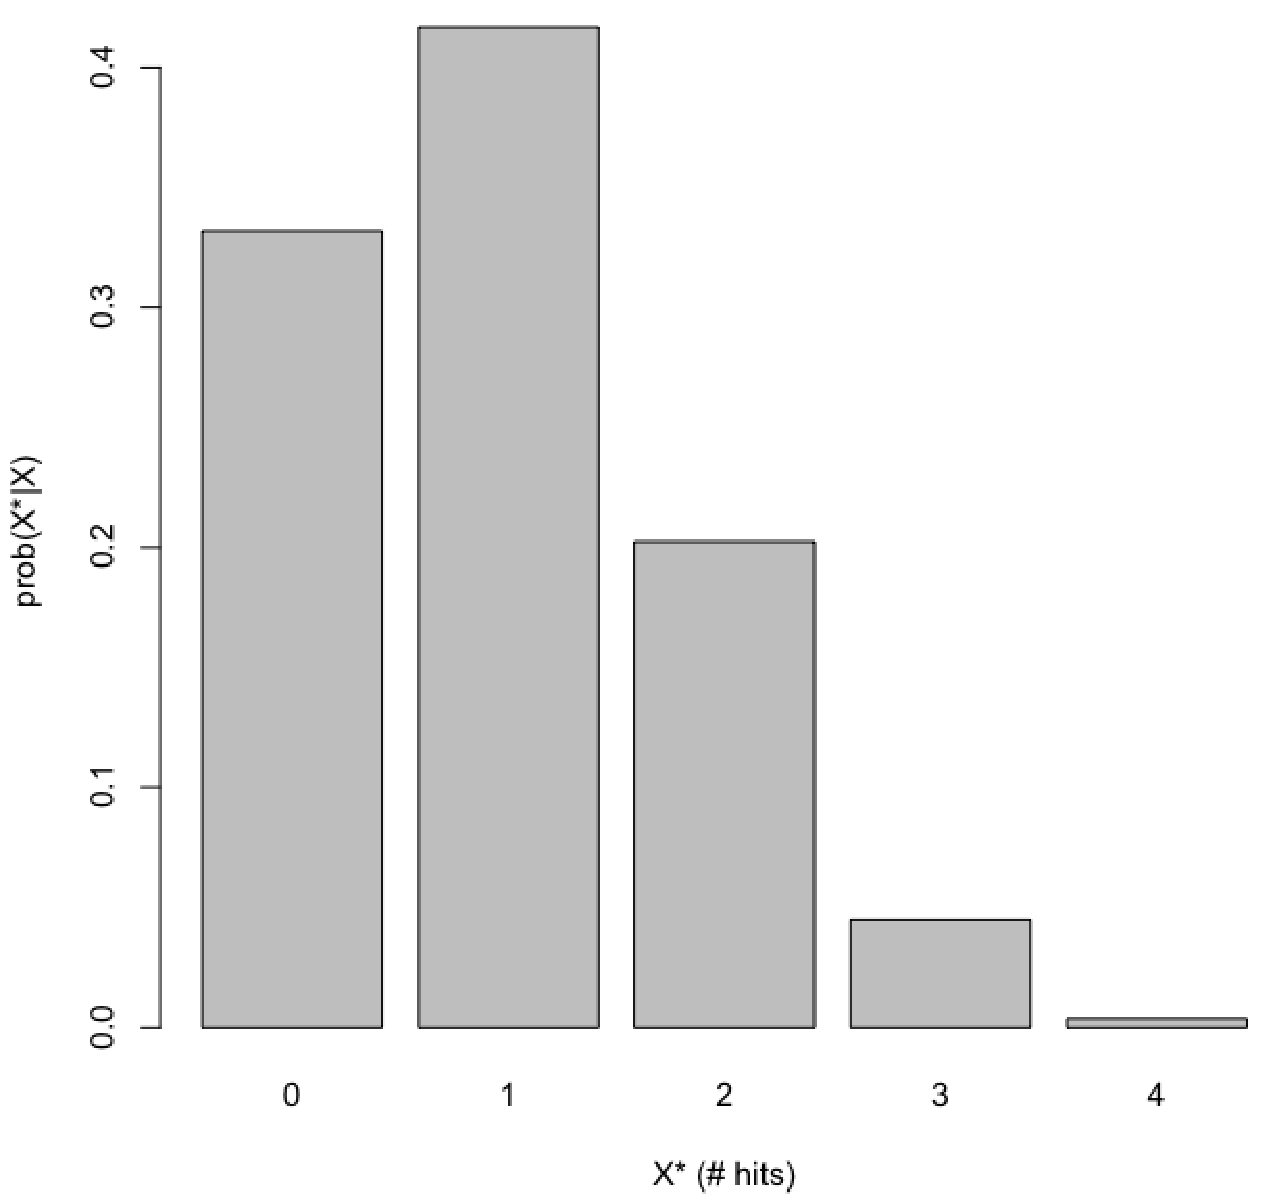
\includegraphics[width=3.0in]{post_pred.pdf}
\end{figure}

Does the data from (b) look abnormal for this model? Yes / no. \spc{0.5}

\subquestionwithpoints{7} Test the following hypotheses by finding an integral or \texttt{R}-language expression for the Bayesian $p$-val for the data in (b) and prior in (o):

\beqn
&& H_0: \theta \geq \theta_0 \\
&& H_a: \theta < \theta_0
\eeqn

where $\theta_0 = \expe{\theta}$. That is, we're testing if this batter is truly \qu{below-average} as compared to the 6,061 career major league baseball players from the official dataset.\spc{8}

\subquestionwithpoints{7} Write an integral or \texttt{R}-language expression for $K$, the Bayes Factor in favor of $H_a$.\spc{9}

\subquestionwithpoints{3} For the model in (a), specify $\mathcal{F}$ (the likelihood model) of a hit at a single at bat. \spc{3}

\subquestionwithpoints{3} [Extra credit] For the the data in (b) and prior in (o), compute $\expesub{X}{\cexpesub{\theta}{\theta}{X}}$ using the Law of Iterated Expectation. \spc{2}

\subquestionwithpoints{3} [Extra credit] For the data in (b), what is the frequentist predictive distribution?

\eenum

\end{document}
